\chapter{Uvod}

\qquad U ovom radu je predstavljeno upravljanje električnim vozilom (slika \ref{fig:buggy}) sa pogonom na sva četiri točka. Proizvođač \href{https://www.qsmotor.com/product/8000w-car-motor/}{motora} je kompanija \textit{QSMOTOR}. Snaga motora je $8000W$, a standardni napon napajanja iznosi $72V$. Svaki od motora je spojen na odgovarajući pretvarač/\href{https://kellycontroller.com/shop/kls-h/}{invertor}. Motori su trofazni i sadrže dva seta Hallovih senzora za određivanje brzine i pozicije. Datasheet motora je dat u prilogu \ref{motor_datasheet}, a dio dokumentacije pretvarača \textit{KLS7275H} u prilogu \ref{kelly_datasheet}. Razvoj upravljačkog prototipa će biti realiziran pomoću \href{https://www.dspace.com/en/inc/home/products/hw/microlabbox.cfm?fbclid=IwAR08_hHwsXPVRs6ng2DLSU5HA3vDNzpBa9CMpO8DWlSQ1DXPK58BkLmoiRE}{dSpace} sistema.

\begin{figure}
\begin{center}
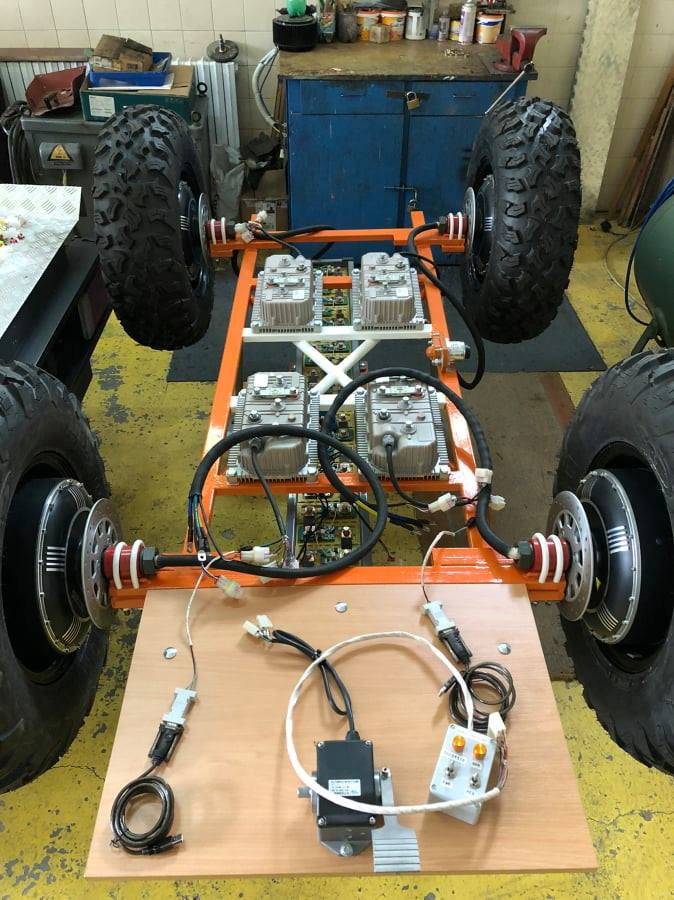
\includegraphics[scale=0.5]{slike/electric_car.jpg}
\end{center}
\caption{Električno $4x4$ vozilo}
\label{fig:buggy}
\end{figure}

\section{Motor}

\qquad Motor je trofazni sa $16$ pari polova, nominalne snage $8000W$. Za mjerenje brzine i pozicije motora, dostupna su dva seta Hallovih senzora. Moguće je mjeriti i temperaturu motora pomoću temperaturnog senzora $KTY83/122$. Motor sadrži dva konektora, čiji pinovi odgovaraju pinovima na \textit{DJ7061Y-2.3-21} konektoru energetskog pretvarača. Svaki od konektora daje informacije sa Hallovog i temperaturnog senzora.

\section{Papučica gasa}

\qquad Brzinu motora je moguće zadavati pomoću papučice gasa. Model koji je odabran ima serijski broj \textit{JKH-005-A-65}. Prema specifikaciji proizvođača \textit{SAYOO}, datoj u prilogu \ref{gas}, dužina kabla spojenog na kočnicu iznosi $65cm$. U kablu se nalazi 5 žica raspoređenih na dva konektora - jedan sa tri, drugi sa četiri žice. Raspon ulaznog i izlaznog napona papučice gasa iznosi od $0$ do $5V$. Ovaj element se konceptualno ponaša kao otpornik sa klizačem koji je spojen na napon napajanja. Izlazni napon otpornika ovisi o položaju klizača, odnosno u ovom slučaju - položaja papučice gasa. Pinovi, prikazani na slici (\ref{fig:gas}), imaju funkcije date u nastavku.

\begin{itemize}
	\item (1) - plus napon napajanja ($5V$)
	\item (2) - minus napon napajanja ($0V$, masa)
	\item (3) - izlazni napon
	\item (4) - izlazni kontakt prekidača
	\item (5) - ulazni kontakt prekidača
\end{itemize}

\begin{figure}
\centering
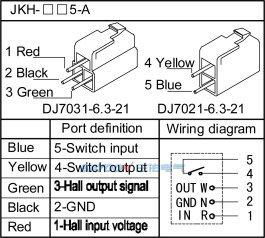
\includegraphics[scale=1]{slike/foot_throttle.png}
\caption{Pinovi papučice gasa}
\label{fig:gas}
\end{figure}

\section{Pretvarač}

\qquad Energetski pretvarač \textit{KLS7275H} proizvođača \textit{Kelly} sadrži 5 digitalnih ulaza: prekidače za gas i kočnicu, prekidače za kretanje naprijed i nazad, te prekidač za \textit{boost} način rada. Dostupna su 3 analogna ulaza: gas, kočnica i temperatura motora. Opseg ulaznog napona može varirati od $0$ do $5V$. Za upravljanje je moguće koristiti i palicu (\textit{engl. joystick}), pri čemu pozicija palice određuje zadanu brzinu i smjer kretanja. \textit{Cruise} režim rada, koji je također dostupan, podrazumijeva zadržavanje zadane brzine vrtnje motora sve dok se ne zada nova brzina ili aktivira kočnica. Pretvarač podržava povezivanje putem \textit{CAN} mreže.

\subsection{Pinovi energetskog pretvarača}

\qquad \textit{KLS7275H} kontroler posjeduje tri konektora prikazana na slici (\ref{fig:kellypins} i 22 pina. Pored standardnih pinova za napajanje, pretvarač posjeduje pinove za prikupljanje informacija sa motora (Hallov senzor i temperaturni senzor), kao i pinove za definiranje smjera i brzine vrtnje motora. Žica spojena na odgovarajući pin je označena jedinstvenom bojom i brojem. Funkcije pinova su date u nastavku.

\begin{itemize}
	\item Konektor \textit{DJ7091Y-2.3-11}
	\begin{itemize}
		\item (14) REV-SW - prekidač za kretanje nazad
		\item \hphantom{0}(6) GND - minus napona napajanja, povratni signal, masa
		\item (12) FWD - prekidač za kretanje naprijed
		\item (11) 12V - naponski izvor od $12V$
		\item (25) 12V Brake - ručna kočnica
		\item (22) ECO - prekidač za štedljivi način rada
		\item (33) CAN-H - \textit{high} pin za CAN komunikaciju
		\item \hphantom{0}(7) PWR - plus napona napajanja pretvarača
		\item (34) CAN-L - \textit{low} pin za CAN komunikaciju
	\end{itemize}
	\item Konektor \textit{DJ7091Y-2.3-21}
		\begin{itemize}
		\item (15) FOOT-SW - prekidač za gas
		\item \hphantom{0}(3) Throttle - analogni ulaz za gas ($0-5V$)
		\item (20) GND - minus napon napajanja, povratni signal, masa
		\item \hphantom{0}(8) Meter - kopija signala sa Hallovog senzora
		\item \hphantom{0}(4) 5V - naponski izvor od $5V$
		\item \hphantom{0}(2) Brake-AN - \textit{boost} funkcija ili analogni ulaz za regenerativni tip kočenja
		\item (11) 12V - naponski izvor od $12V$
	\end{itemize}
	\item Konektor \textit{DJ7061Y-2.3-21}
		\begin{itemize}
		\item (21) GND - minus napon napajanja, povratni signal, masa
		\item \hphantom{0}(1) Temp - temperatura motora
		\item \hphantom{0}(5) 5V - naponski izvor od $5V$
		\item (18) Hall A - signal Hallovog senzora za fazu A
		\item (17) Hall B - signal Hallovog senzora za fazu B 
		\item (16) Hall C - signal Hallovog senzora za fazu C 
	\end{itemize}
\end{itemize}

\begin{figure}
\begin{center}
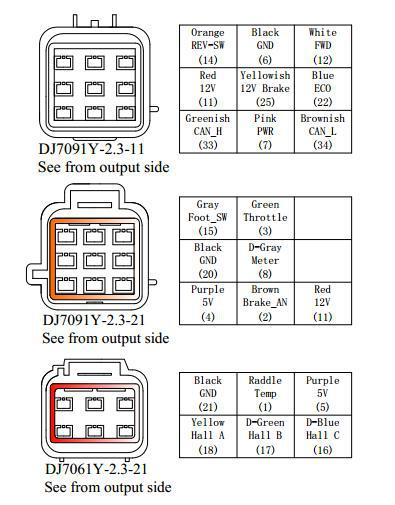
\includegraphics[scale=1]{slike/kellypins.jpg}
\end{center}
\caption{Pinovi \textit{Kelly KLS7275H} pretvarača}
\label{fig:kellypins}
\end{figure}

\section{Upravljanje motorom}

\qquad Energetski pretvarač/kontroler koristi vektorsku modulaciju (\textit{engl. space-vector modulation}) za upravljanje trofaznim motorom. Za upravljanje cjelokupnim sistemom vozila, potrebno je uključiti dodatni sloj upravljanja, koji će upravljati paralelno sa svim pretvaračima koji su povezani sa motorima.

Za sada će konceptualno biti razmotreno upravljanje jednim motorom. Shema upravljanja je data na sljedećoj strani. Osnovna ideja upravljanja se zasniva na tome da se na pin (3) \textit{KLS7275H} pretvarača dovodi signal u rasponu od $0$ do $5V$, koji će proporcionalno svojoj vrijednosti - određivati željenu brzinu vrtnje motora. Izvor signala gasa može biti potenciometar ili nožna papučica, što se također mora uzeti u obzir prilikom konfiguracije samog pretvarača. U prikazanoj konfiguraciji je potrebno obezbjediti signal koji će na pinu (15) davati informaciju o stanju papučice gasa. Funkcija analognog regenerativnog kočenja se može realizirati na sličan način, pri čemu za razliku od gasa, nije potrebna infromacija da li je papučica aktivirana. Na pinu (25) je moguće realizirati $12V$ ručnu kočnicu.

Korisnik može mijenjati smjer vrtnje motora, odnosno smjer kretanja vozila (naprijed ili nazad) dovođenjem odgovarajuće kombinacije signala na pinove (12) i (14). Na osnovu ulaznih signala, energetski pretvarač pokreće trofazni DC motor bez četkica. Pinovi (16), (17) i (18) služe za prikupljanje signala sa Hallovog senzora na samom motoru. Napajanje Hallovog senzora iznosi $5V$.

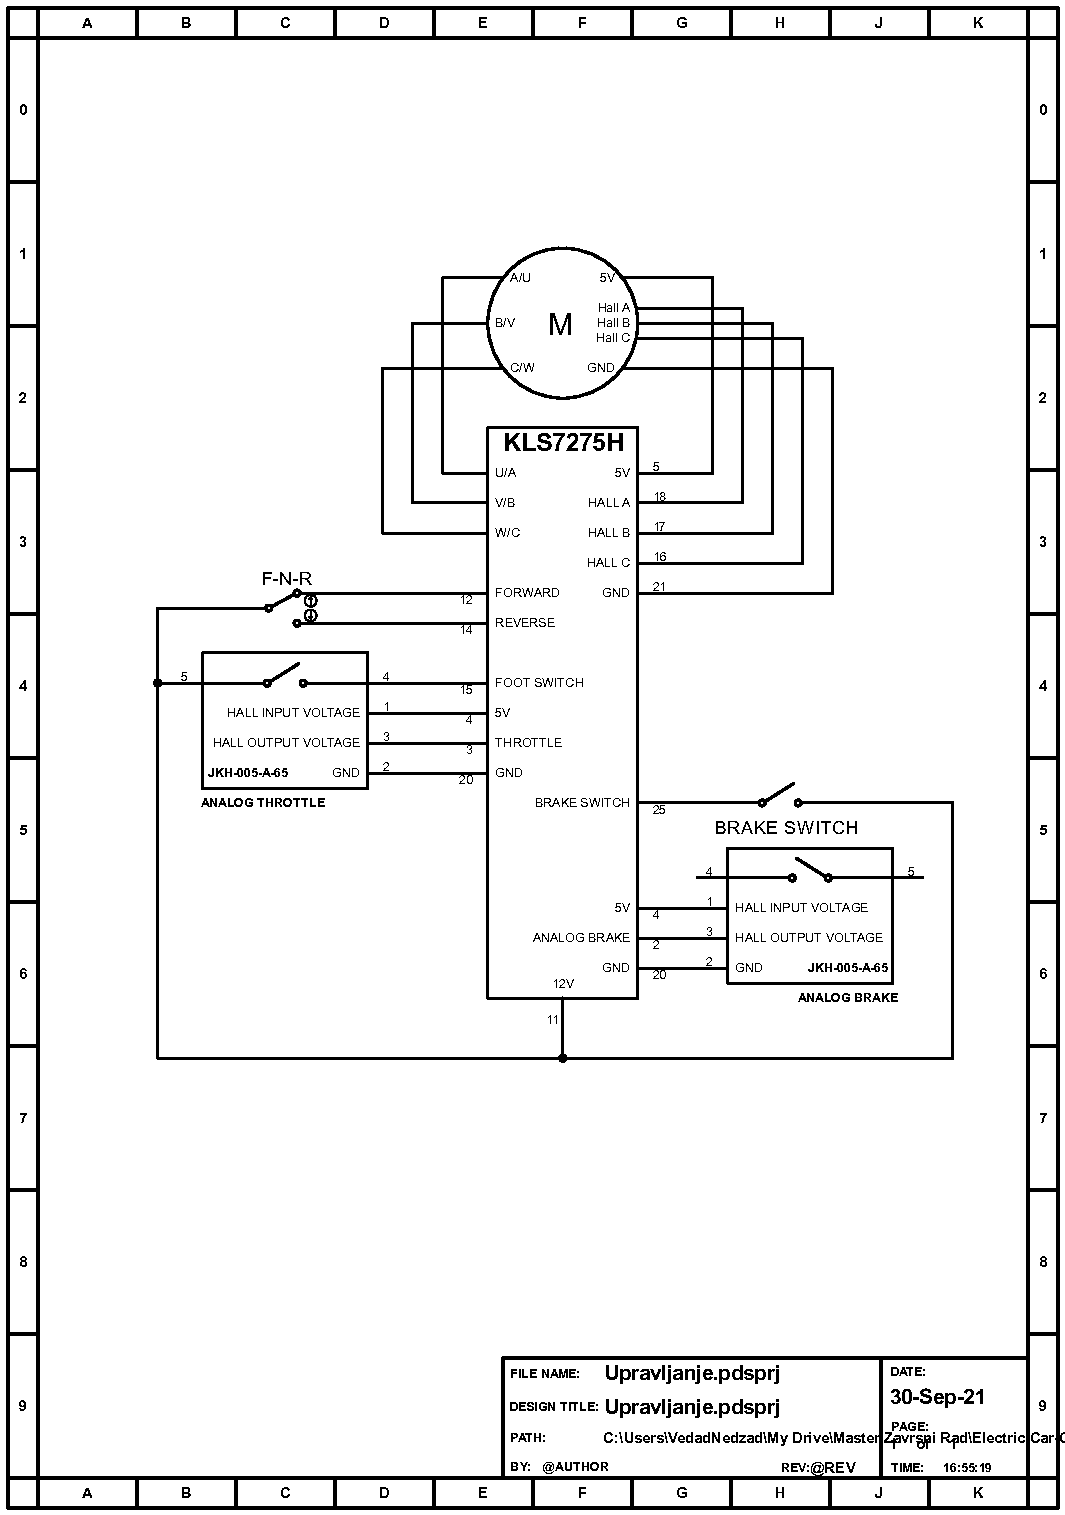
\includepdf[pages=-]{dokumenti/proteus upravljanje}


\begin{comment}

\begin{table}[]
\centering
\begin{tabular}{|c|c|c|c|c|c|}
\hline
\multicolumn{2}{|c|}{Configuration} & \multicolumn{3}{c|}{Pin Status} & \multirow{2}{*}{Running Status} \\ \cline{1-5}
Forward Switch & Foot Switch & FWD-SW (12) & REV-SW (14) & FOOT (15) &  \\ \hline
\multirow{4}{*}{Enable} & \multirow{4}{*}{Disable} & OFF & OFF & X & Neutral \\ \cline{3-6} 
 &  & OFF & ON & X & Reverse \\ \cline{3-6} 
 &  & ON & OFF & X & Forward \\ \cline{3-6} 
 &  & ON & ON & X & Neutral \\ \hline
\multirow{4}{*}{Disable} & \multirow{4}{*}{Enable} & X & OFF & OFF & Can't operate \\ \cline{3-6} 
 &  & X & ON & OFF & Can't operate \\ \cline{3-6} 
 &  & X & ON & ON & Reverse \\ \cline{3-6} 
 &  & X & OFF & ON & Forward \\ \hline
\multirow{2}{*}{Disable} & \multirow{2}{*}{Disable} & X & OFF & X & Forward \\ \cline{3-6} 
 &  & X & ON & X & Reverse \\ \hline
\end{tabular}
\caption{Konfiguracija pretvarača}
\label{tab:konfiguracija}
\end{table}

\end{comment}

\section{Konfiguracija parametara pretvarača}

\qquad Parametre \textit{KLS7275H} kontrolera je moguće podešavati pomoću PC ili Android uređaja. Veza sa PC uređajem se ostvaruje preko \textit{USB-RS232} konektora. Softver za konfiguraciju je dostupan na zvaničnoj \href{https://kellycontroller.com/shop/kls-h/}{stranici} proizvođača. Dijaloški okvir programa je prikazan na slici (\ref{fig:configuration}). Podešavanja vezana za motor i samo vozilo koje će motor pogoniti kao dio sistema su odvojena. Informacije kao što su ime modula, serijski broj, verzija softvera i napon pretvarača su dostupna samo za čitanje.

\begin{figure}
\centering
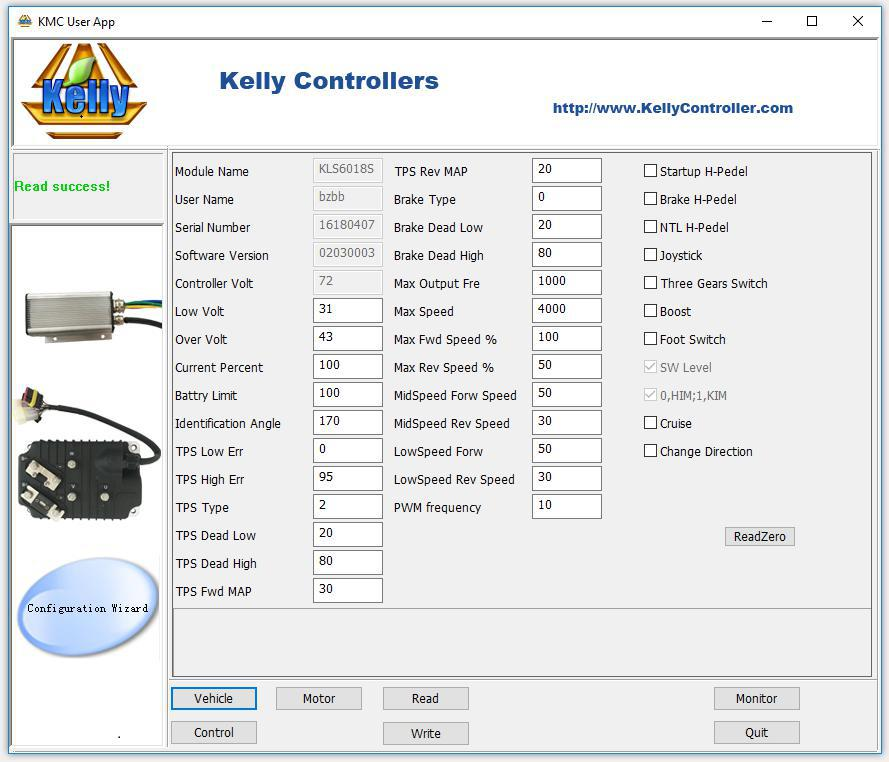
\includegraphics[width=\textwidth]{slike/configuration.jpg}
\caption{Program za konfiguraciju energetskog pretvarača}
\label{fig:configuration}
\end{figure}

\section{Operacija identifikacije ugla}

\qquad Prije puštanja određenog motora u rad, potrebno izvršiti proceduru \textit{identifikacije ugla}. Ova operacija se izvršava korištenjem aplikacije na računaru koji je povezan sa energetskim pretvaračem preko \textit{USB-RS232} konektora. Shema spajanja je data na slici (\ref{fig:angleident}). Pretvarač je spojen na motor sa tri faze, a sa motora se prenosi signal sa Hallovog senzora. Vanjski element za zadavanje gasa također treba povezati sa pretvaračem, pri čemu taj element može jednostavno biti potenciometar ili papučica gasa.

\begin{figure}
\centering
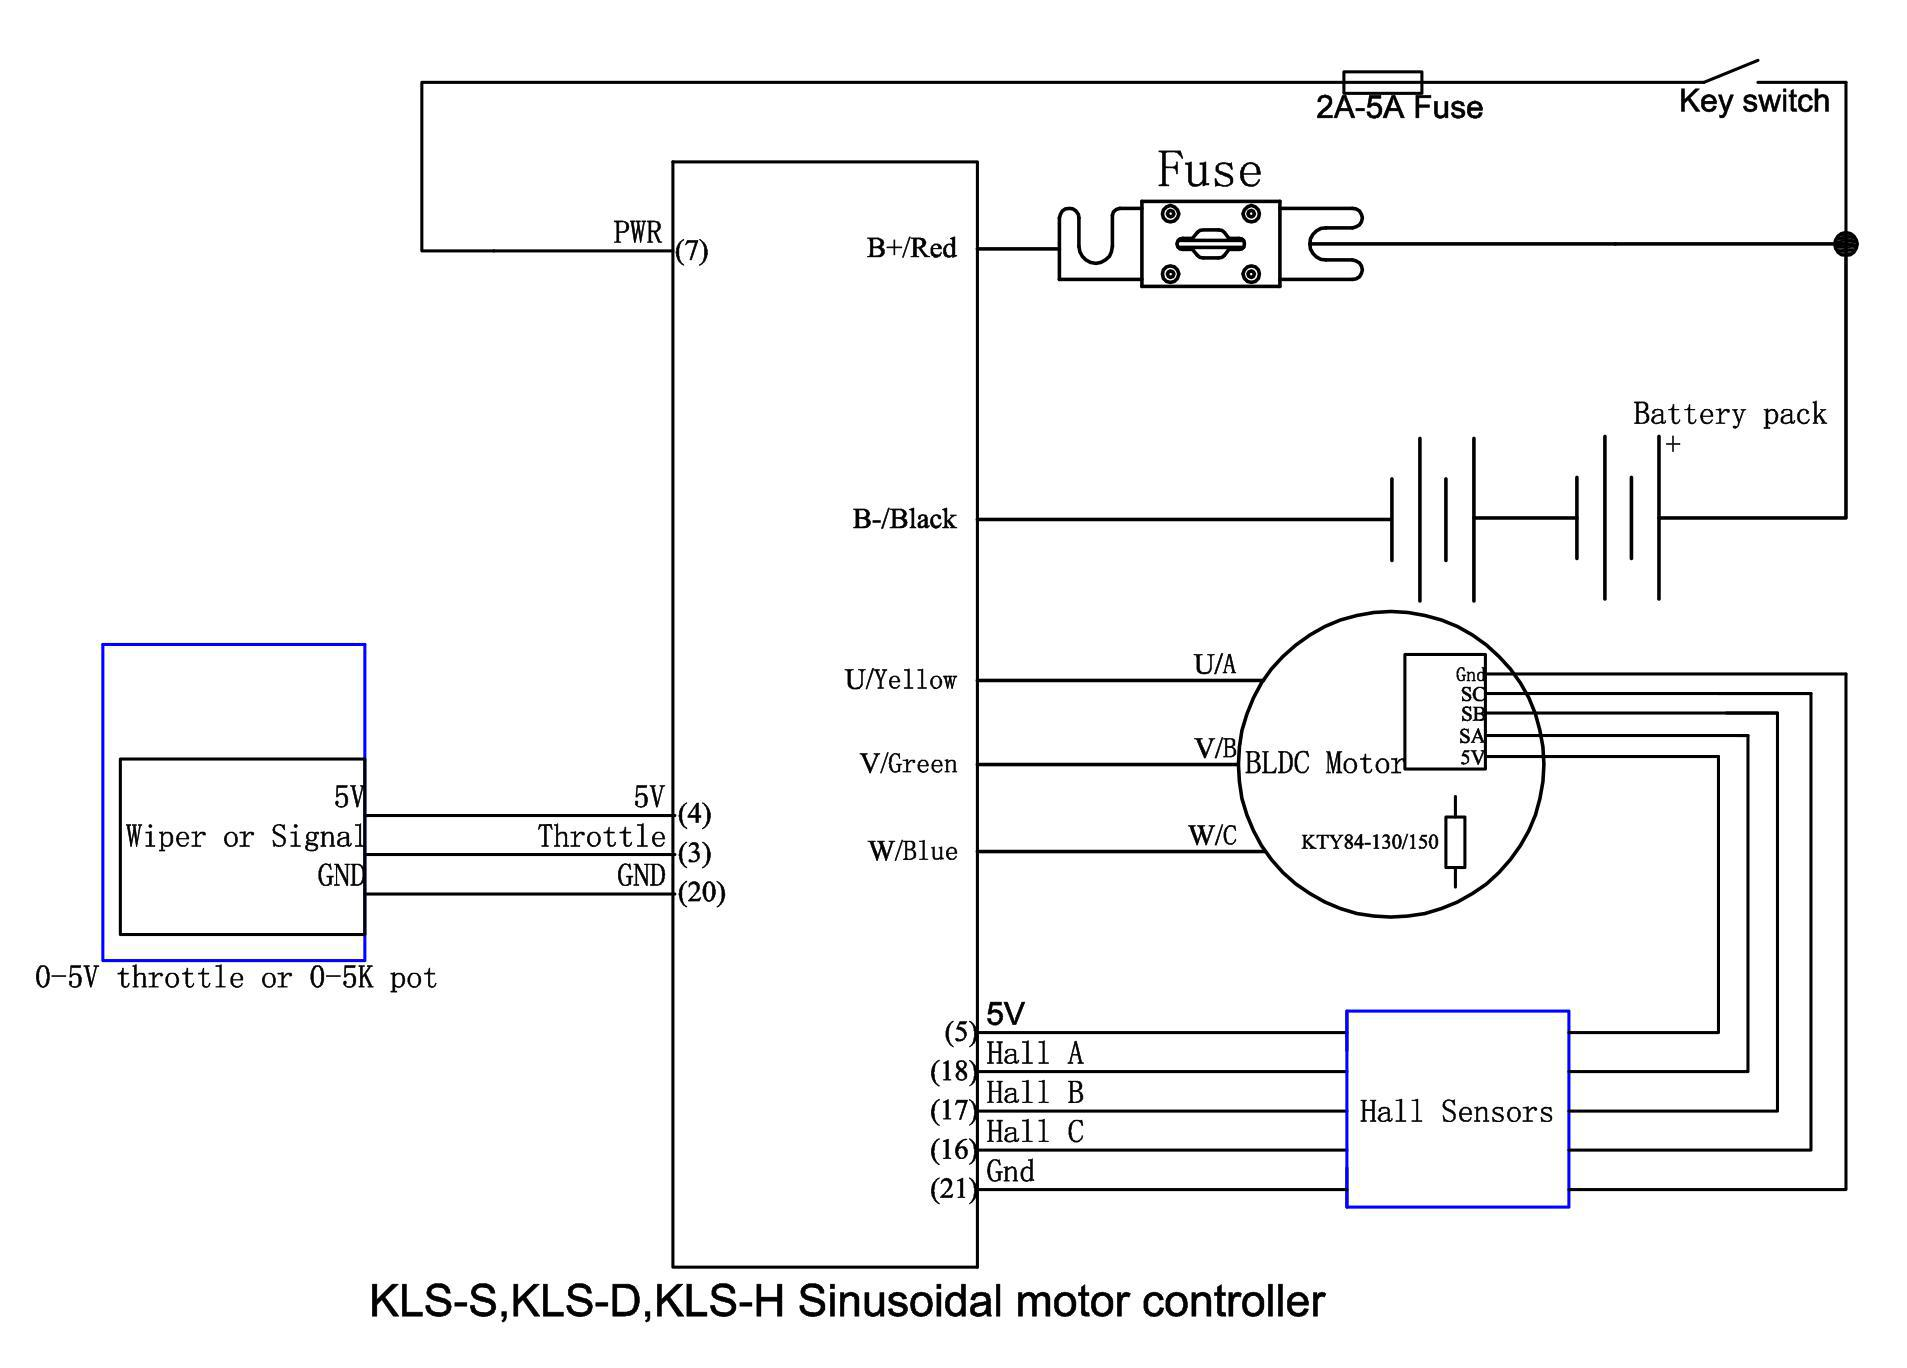
\includegraphics[width=\textwidth]{slike/angleident.jpg}
\caption{Shema spajanja za operaciju identifikacije ugla}
\label{fig:angleident}
\end{figure}

Komponenta koja se može koristiti u tu svrhu je \textit{Controller Control Box}, prikazana na slici (\ref{fig:controlbox}). Shema spajanja sa kontrolerom preko 14-pinskog konektora je data u prilogu \ref{control}, pri čemu je za realizaciju identifikacije ugla dovoljno koristiti opciju u kojoj se \textit{PWR} prekidač na kontrolnoj kutiji koristi za \textit{Key switch} na slici (\ref{fig:angleident}) i konfiguracija \textit{Throttle} potenciometra kao element zadavanja gasa.

\begin{figure}
\centering
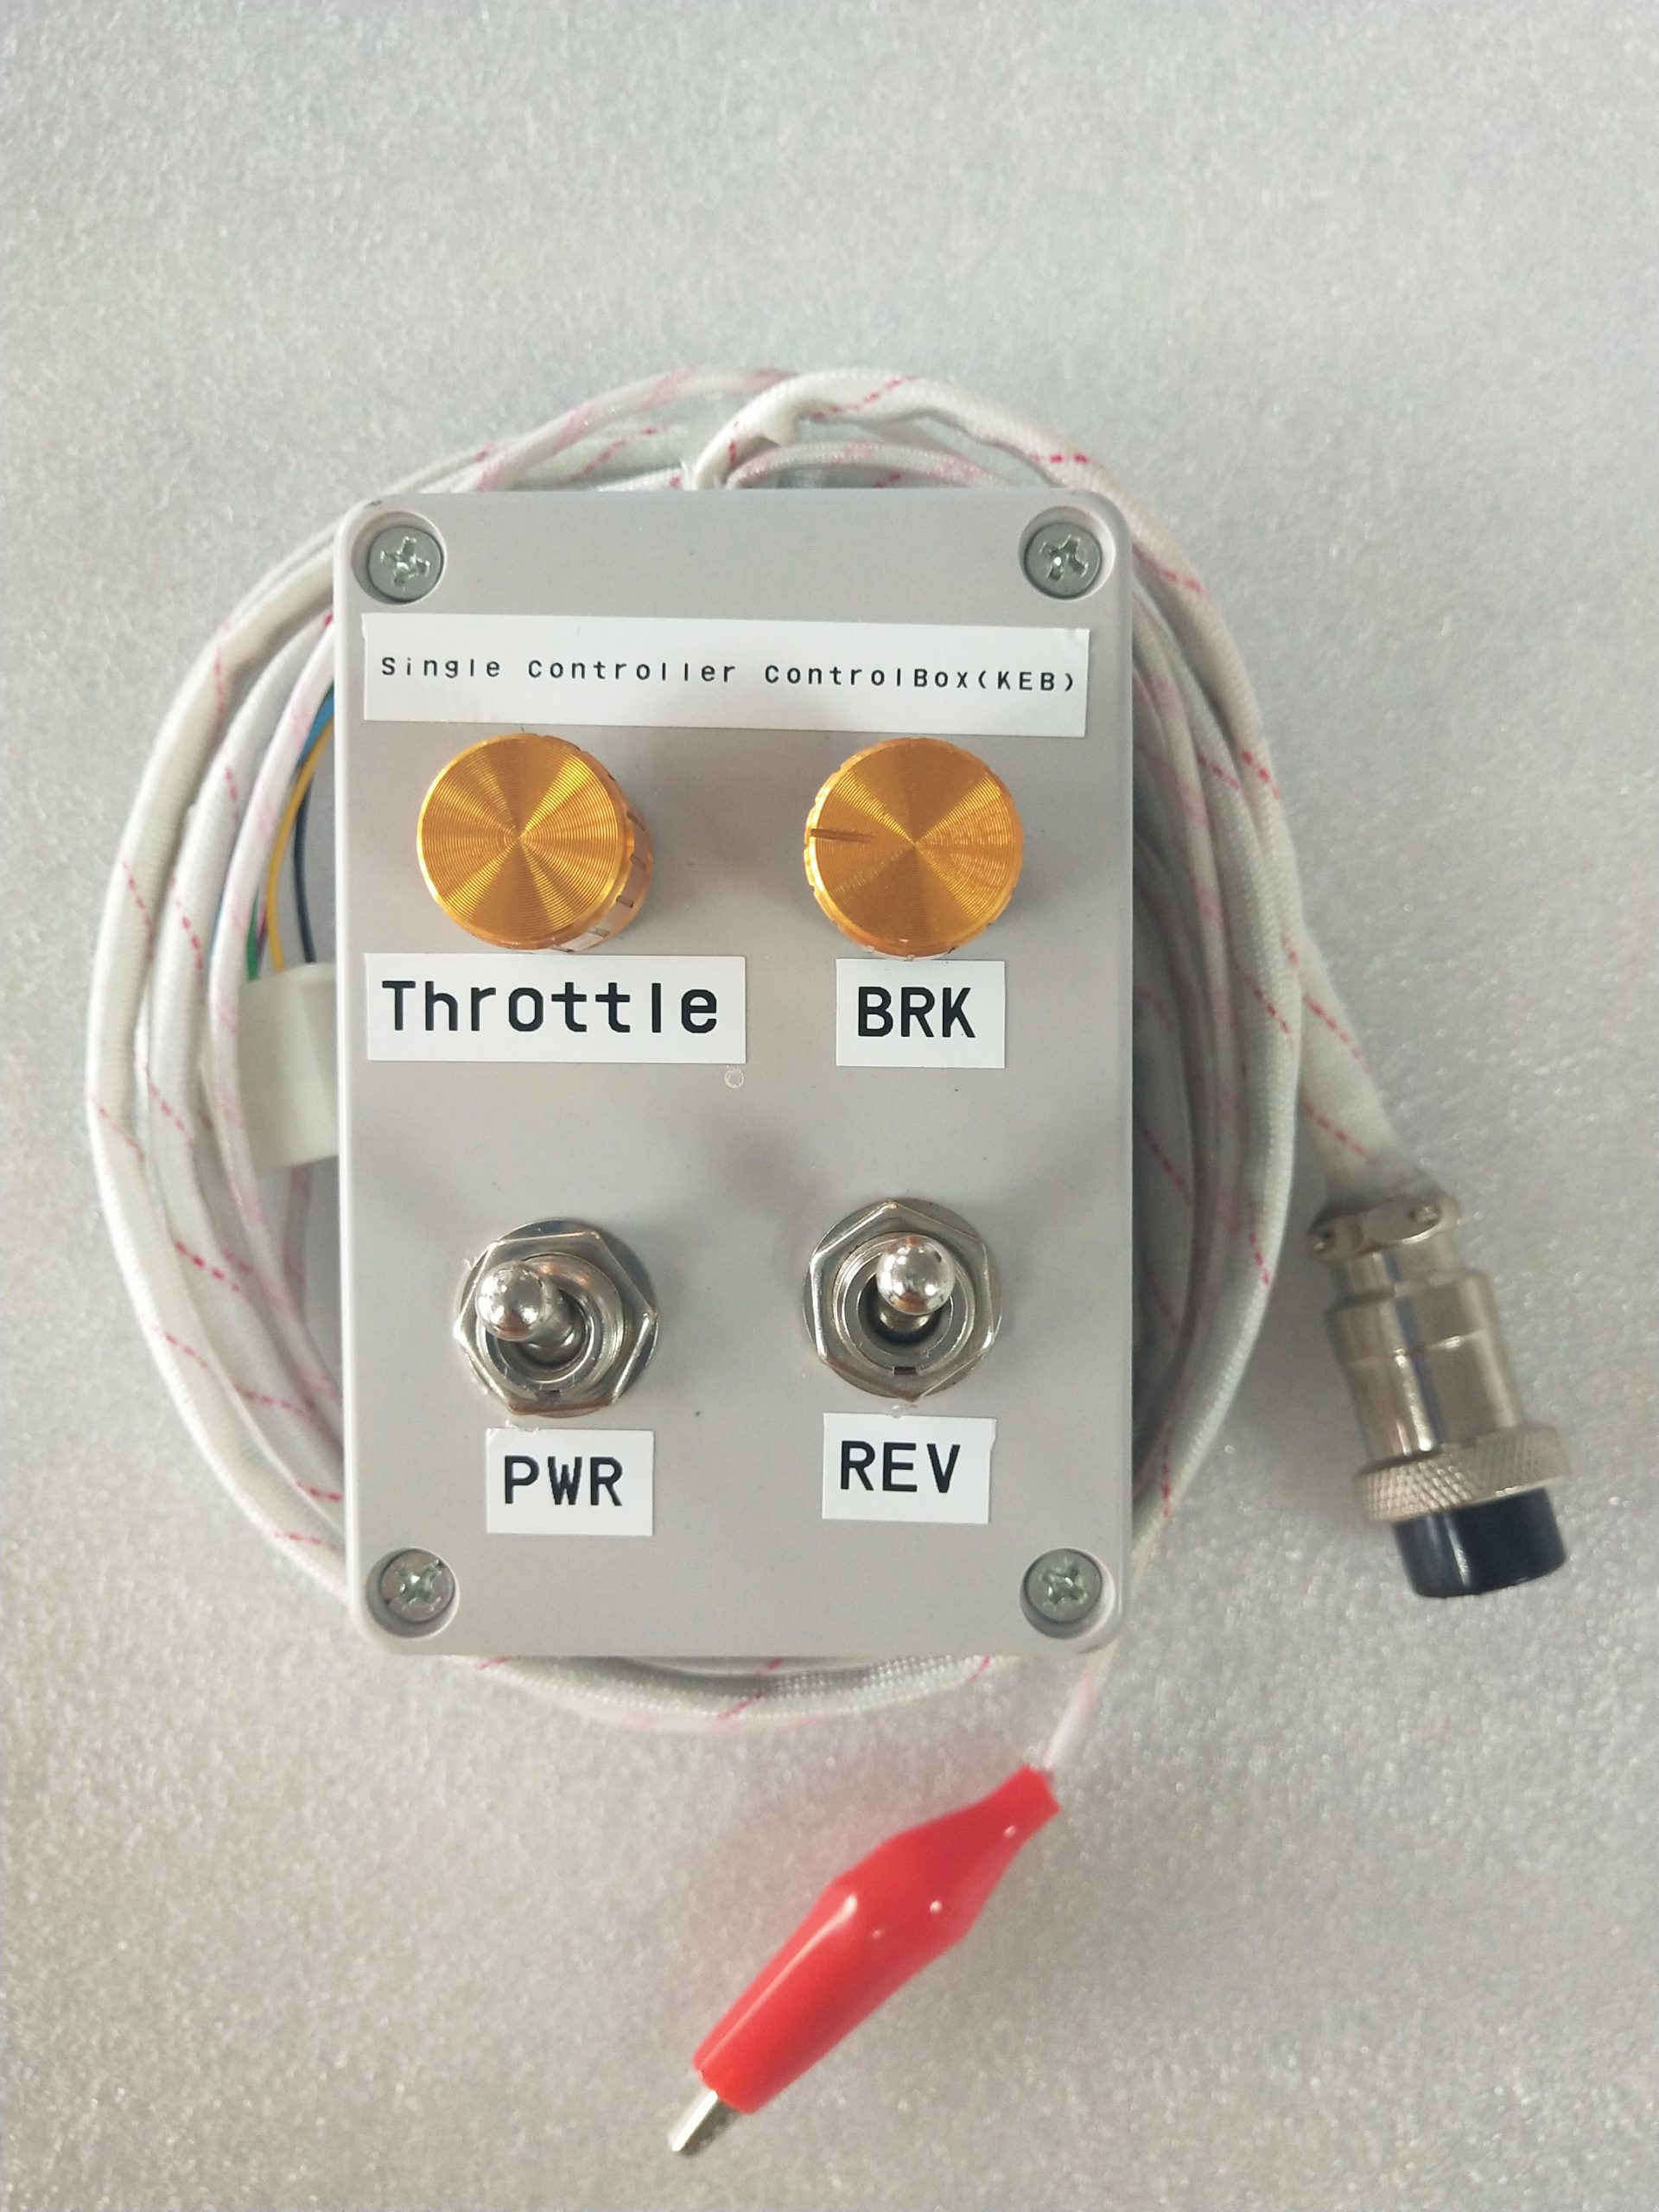
\includegraphics[scale=0.1]{slike/controlbox.jpg}
\caption{Controller Control Box}
\label{fig:controlbox}
\end{figure}

Pri povezivanju svih elemenata potrebno je da \textit{PWR} prekidač, odnosno\textit{Key switch} bude u otvorenom stanju. Nakon što se preuzme softver za konfiguraciju i instalira na PC, prekidač za napajanje je potrebno zatvoriti i pokrenuti instalirani softver. Kada se otvori dijaloški prozor programa (slika \ref{fig:configuration}), potrebno je kliknuti na opciju \textit{Read}.

Naredni korak u postupku identifikacije ugla je upisivanje broja \textbf{170} u parametar \textit{Identification Angle} i odabir opcije \textit{Write}. Zatim je potrebno izaći iz programa za konfiguraciju. Isključivanjem dovoda napajanja na nekoliko sekundi i ponovnim spuštanjem \textit{PWR} prekidača, motor započinje kretanje nasumično u oba smjera. Proces identifikacije traje od 2 do 3 minute.

Kada se proces završi, pretvarač će dati $3-2$ kod greške - zujalica (\textit{engl. buzzer}) će najprije dati 3, a zatim 2 brza zvučna signala. Zatim je potrebno opet na nekoliko sekundi isključiti napajanje kontrolera. Nakon ponovnog pokretanja korisničkog sučelja za konfiguraciju kontrolera, potrebno je provjeriti \textit{Identification Angle} parametar, ukoliko je proces identifikacije uspješno izvršen - parametar ima vrijednost 85.

Iako se u procesu identifikacije ugla nije koristio potenciometar za davanje gasa, ovaj element služi za provjeru da li se motor kreće u željenom smjeru. Ukoliko to nije slučaj, potrebno je označiti (\textit{engl. check}) opciju \textit{Change Direction} u programu za konfiguraciju. Da bi se promjena sačuvala potrebno je kliknuti na dugme \textit{Write} i resetirati napajanje.


